\documentclass{standalone}
\usepackage{amsmath, amsfonts, amsthm}
\usepackage{siunitx}
\usepackage{graphicx}
\usepackage{tikz}
\usepackage{circuitikz}
\usetikzlibrary{patterns}
\usepackage{scalerel}
\usepackage{pict2e}
\usepackage{tkz-euclide}
\usetikzlibrary{calc}
\usetikzlibrary{arrows.meta}
\usetikzlibrary{shadows}
\usetikzlibrary{external}
\usetikzlibrary{decorations.pathmorphing}
\usetikzlibrary{shapes.geometric}
\usetikzlibrary{arrows,shapes.gates.logic.US,shapes.gates.logic.IEC,calc}
\usepackage{pgfplots}
\pgfplotsset{compat=newest}
\usepgfplotslibrary{statistics}
\usepgfplotslibrary{fillbetween}

\begin{document}
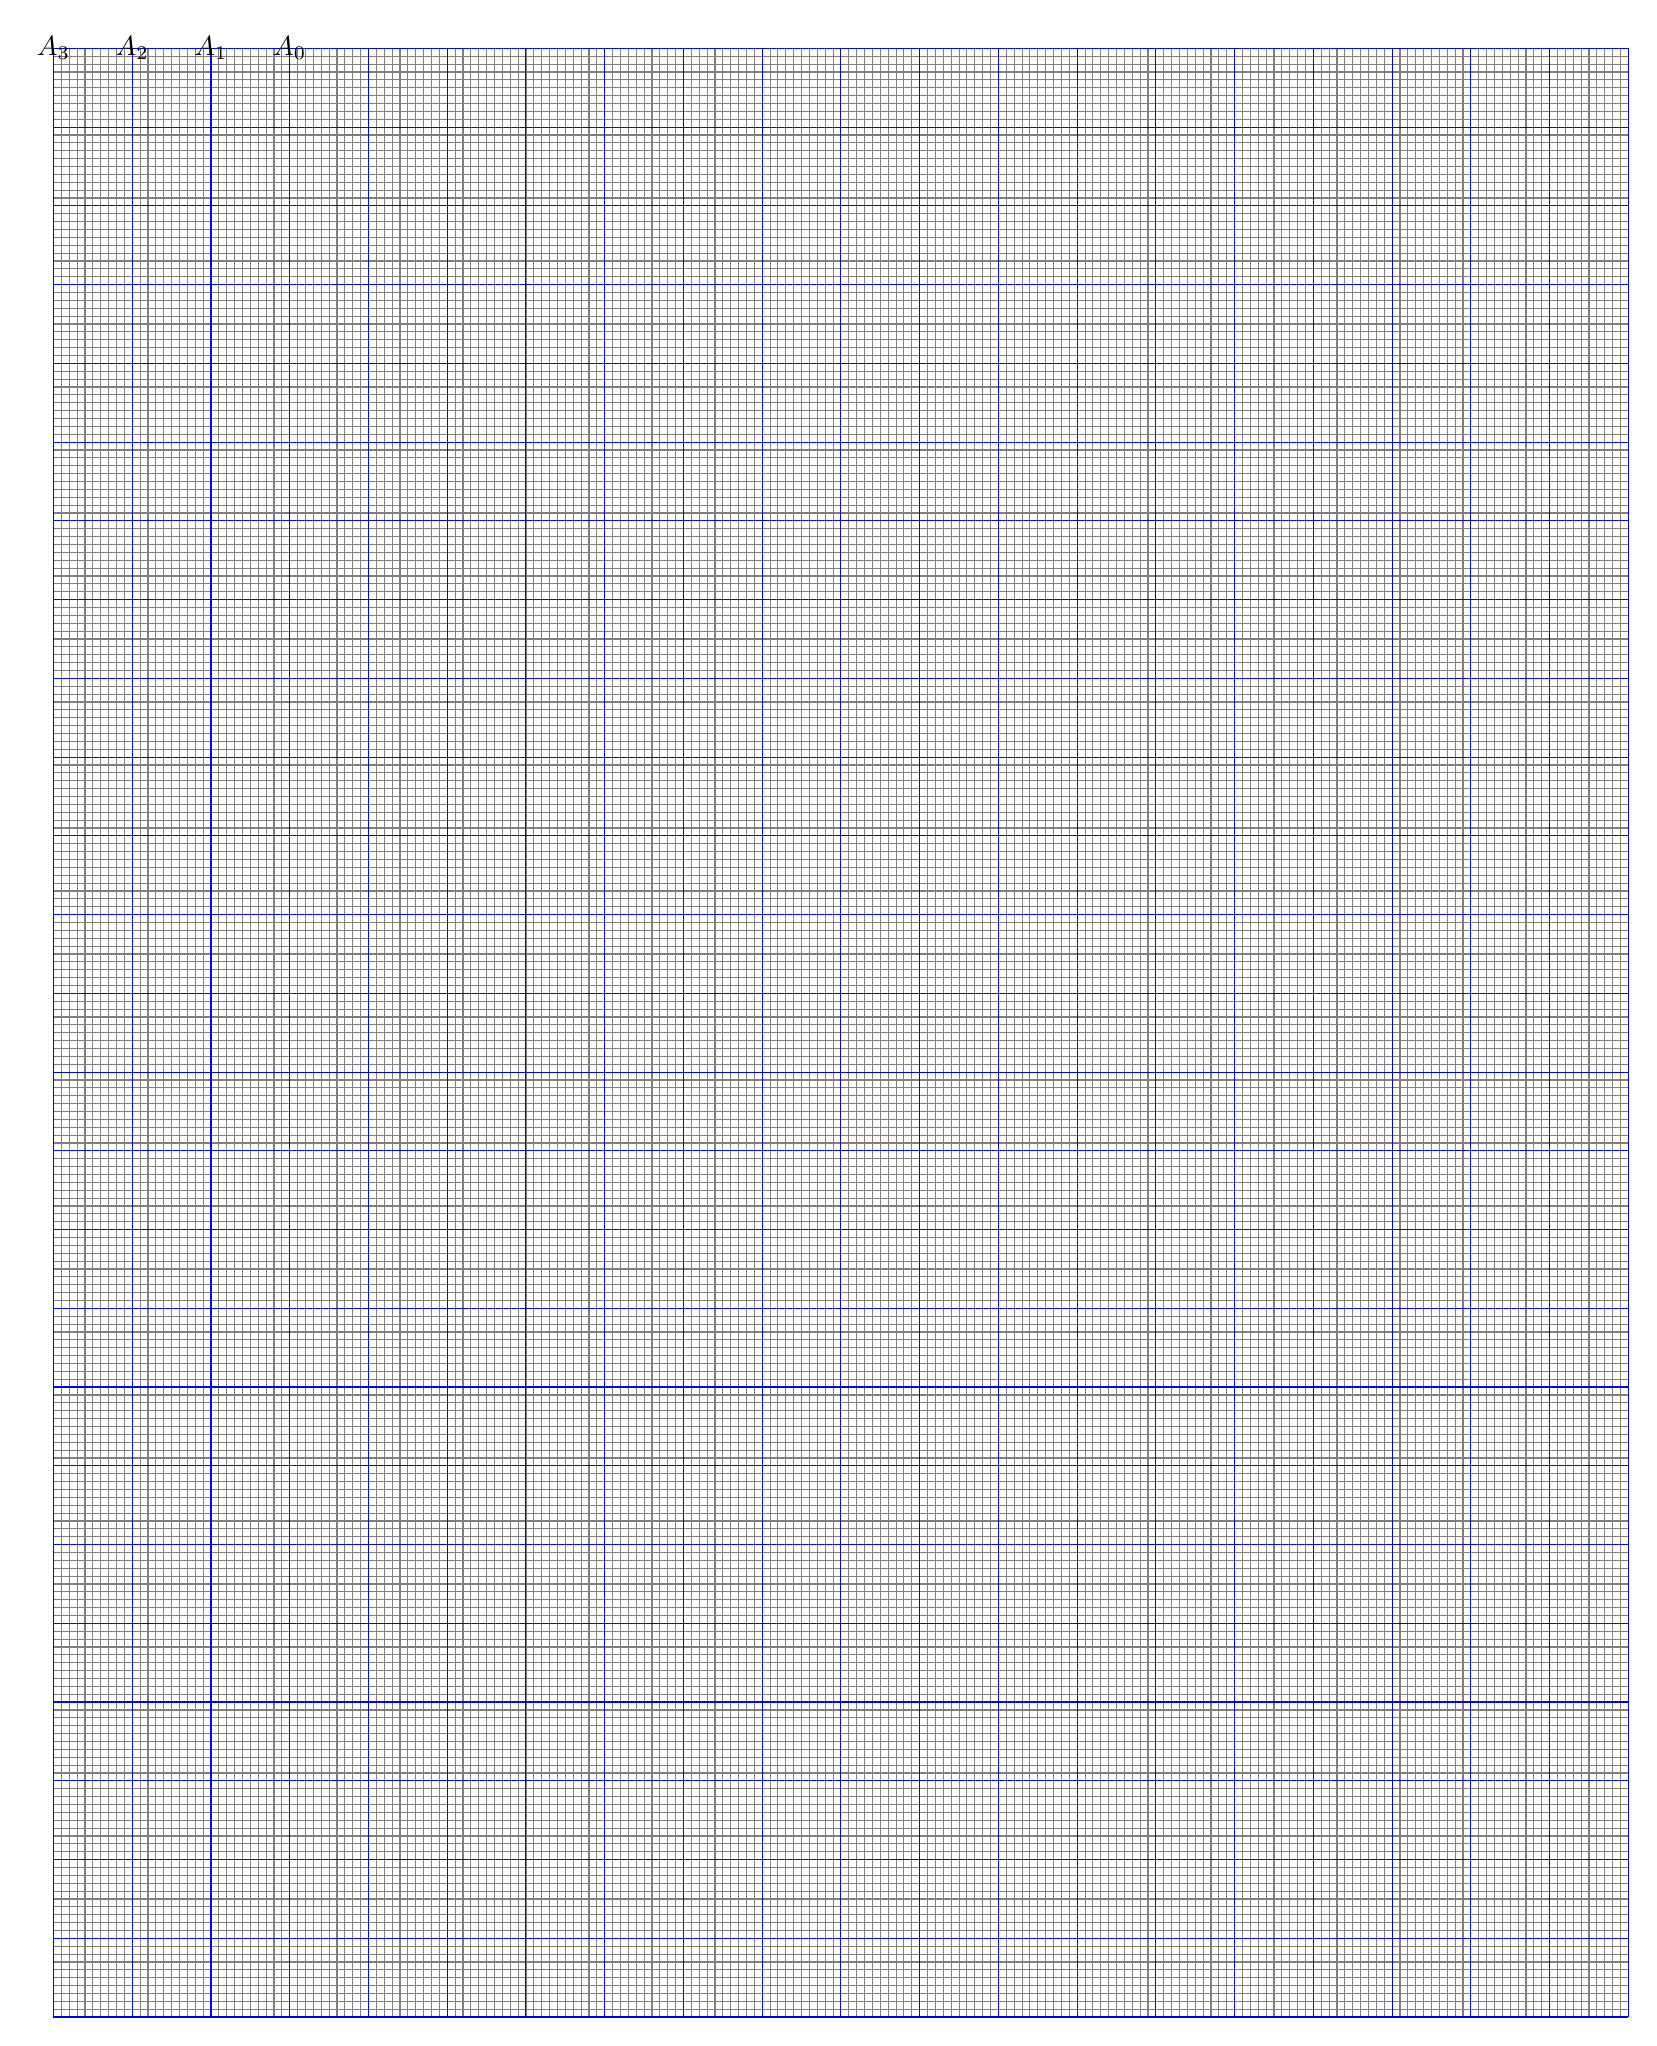
\begin{tikzpicture}
	\draw [help lines, step=0.1, gray] (0,0) grid (20, -25);
	\draw [help lines, blue] (0,0) grid (20,-25);

	\node (A3) at (0,0)      {$A_3$};
	\node (A2) [right of=A3] {$A_2$};
	\node (A1) [right of=A2] {$A_1$};
	\node (A0) [right of=A1] {$A_0$};

\end{tikzpicture}
\end{document}
